\documentclass[../00_main.tex]{subfiles}

\begin{document}

\section{Class 08.09.2020}

\subsection{Present Value and Discount}

\subsubsection{Present Value}

\begin{itemize}
    \item we define the \textit{present value $t$ years in the past} as the
        amount of money that will accumulate to the principal in $t$ years
    \item this is the reverse of what we have been calculating thus far\\
        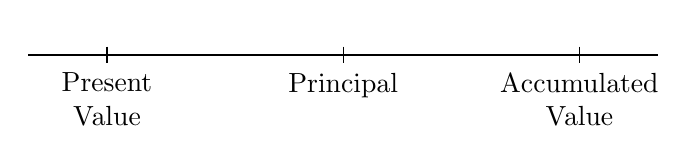
\begin{tikzpicture}
            \draw (0,0) -- (8,0);
            \foreach \x in {1,4,7}
              \draw (\x cm,3pt) -- (\x cm,-3pt);
            \draw (1,0) node[below=3pt, align=center] {Present\\Value}
                node[above=3pt] {$ $};
            \draw (4,0) node[below=3pt, align=center] {Principal};
            \draw (7,0) node[below=3pt, align=center] {Accumulated\\Value};
        \end{tikzpicture}
    \item $v$ is the amount of money needed to accumulate to 1 within 1 year
        \begin{equation}\nonumber
            v = \frac{1}{1+i}
        \end{equation}
    \item how $v$ works can be seen in this timeline that shows the evolution
        of $a(t)$\\
        \begin{tikzpicture}
            \draw (0,0) -- (8,0);
            \foreach \x in {1,4,7}
              \draw (\x cm,3pt) -- (\x cm,-3pt);
            \draw (1,0) node[below=3pt] {$-1$} node[above=3pt] {$\frac{1}{1+i}$};
            \draw (4,0) node[below=3pt] {$0$} node[above=3pt] {$1$};
            \draw (7,0) node[below=3pt] {$1$} node[above=3pt] {$1+i$};
        \end{tikzpicture}
    \item for compound interest, $v$ is
        \begin{equation}
            v^t = \frac{1}{(1+i)^t}
        \end{equation}
    \item this is simply an inverted formula of $a(t)$ for compound interest
    \item for simple interest the present value is called $x$
        \begin{equation}\nonumber
            x = \frac{1}{1+it}
        \end{equation}
\end{itemize}

\subsubsection{Discount}

\begin{itemize}
    \item imagine \$100 was invested and accumulated to \$112 in 1 year
    \item \$100 was the starting figure and interest (\$12) was added to it
    \item we could look at it the other way around and say \$112 is the
        starting value and at the start of the year \$12 was subtracted from it
    \item \$12 here is an amount of \textit{discount}
    \item it's the same as interest, only the point of view is different
    \item discount focuses on the end of the year, so it is defined as
        \begin{equation}\nonumber
            d = \frac{a(1) - 1}{a(1)}
        \end{equation}
    \item this only differs from the definition of $i$ in the denominator,
        which is $a(0)$ for $i$ because the beginning of the year is the focus
    \item effective rate of discount in the $n$th year is
        \begin{equation}\nonumber
            d_n = \frac{a(n) - a(n-1)}{a(n)}
        \end{equation}
    \item some identities relating to $i$ are
        \begin{equation}\nonumber
            \begin{aligned}
                d &< i                  \\
                d &= \frac{i}{1+i}      \\
                1 - d &= v              \\
                i &= \frac{d}{1-d}
            \end{aligned}
        \end{equation}
    \item now the rules for finding the present and accumulated values are
        reversed
        \begin{equation}\nonumber
            \begin{aligned}
                \text{present value}: \qquad &(1-d)^t   \\
                \text{accumulated value}: \qquad &\frac{1}{(1-d)^t}
            \end{aligned}
        \end{equation}
\end{itemize}

\end{document}
